\documentclass{standalone}
\usepackage{pgfplots}
\pgfplotsset{compat=1.18}
\usepgfplotslibrary{groupplots,fillbetween}
\begin{document}
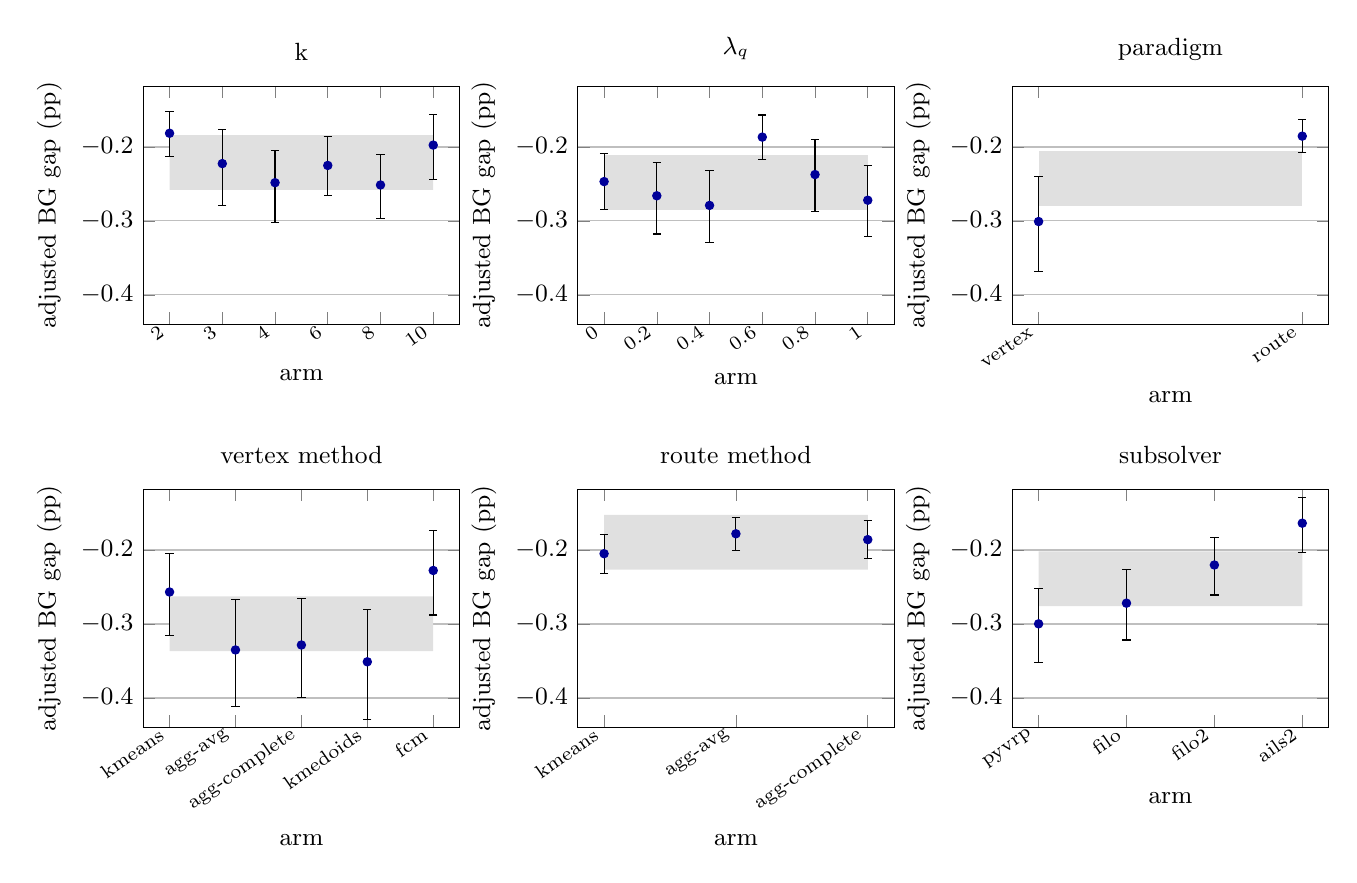
\begin{tikzpicture}
\begin{groupplot}[
  group style={group size=3 by 2, horizontal sep=1.5cm, vertical sep=2.1cm},
  width=5.6cm, height=4.6cm,
  ymin=-0.4396, ymax=-0.1184,
  xlabel={arm},
  ylabel={adjusted BG gap (pp)},
  tick label style={font=\small},
  xticklabel style={rotate=35, anchor=east, font=\scriptsize},
  label style={font=\small},
  title style={font=\small},
  ymajorgrids,
]
\nextgroupplot[title={k}, symbolic x coords={2,3,4,6,8,10}, xtick=data]
\addplot[name path=lo, draw=none, forget plot] coordinates {(2, -0.2580) (3, -0.2580) (4, -0.2580) (6, -0.2580) (8, -0.2580) (10, -0.2580)};
\addplot[name path=hi, draw=none, forget plot] coordinates {(2, -0.1840) (3, -0.1840) (4, -0.1840) (6, -0.1840) (8, -0.1840) (10, -0.1840)};
\addplot[forget plot, fill=black!12, draw=none] fill between[of=lo and hi];
\addplot[only marks, mark=*, mark size=1.5pt, blue!60!black,
  error bars/.cd, y dir=both, y explicit, error bar style={black, thin},
  /pgfplots/.cd] coordinates {(2, -0.1815) += (0, 0.0294) -= (0, 0.0314) (3, -0.2225) += (0, 0.0456) -= (0, 0.0563) (4, -0.2483) += (0, 0.0433) -= (0, 0.0533) (6, -0.2250) += (0, 0.0395) -= (0, 0.0412) (8, -0.2514) += (0, 0.0406) -= (0, 0.0454) (10, -0.1975) += (0, 0.0408) -= (0, 0.0463)};
\nextgroupplot[title={$\lambda_q$}, symbolic x coords={0,0.2,0.4,0.6,0.8,1}, xtick=data]
\addplot[name path=lo, draw=none, forget plot] coordinates {(0, -0.2849) (0.2, -0.2849) (0.4, -0.2849) (0.6, -0.2849) (0.8, -0.2849) (1, -0.2849)};
\addplot[name path=hi, draw=none, forget plot] coordinates {(0, -0.2109) (0.2, -0.2109) (0.4, -0.2109) (0.6, -0.2109) (0.8, -0.2109) (1, -0.2109)};
\addplot[forget plot, fill=black!12, draw=none] fill between[of=lo and hi];
\addplot[only marks, mark=*, mark size=1.5pt, blue!60!black,
  error bars/.cd, y dir=both, y explicit, error bar style={black, thin},
  /pgfplots/.cd] coordinates {(0, -0.2468) += (0, 0.0376) -= (0, 0.0377) (0.2, -0.2660) += (0, 0.0453) -= (0, 0.0516) (0.4, -0.2790) += (0, 0.0469) -= (0, 0.0499) (0.6, -0.1867) += (0, 0.0299) -= (0, 0.0302) (0.8, -0.2373) += (0, 0.0469) -= (0, 0.0500) (1, -0.2720) += (0, 0.0471) -= (0, 0.0490)};
\nextgroupplot[title={paradigm}, symbolic x coords={vertex,route}, xtick=data]
\addplot[name path=lo, draw=none, forget plot] coordinates {(vertex, -0.2801) (route, -0.2801)};
\addplot[name path=hi, draw=none, forget plot] coordinates {(vertex, -0.2061) (route, -0.2061)};
\addplot[forget plot, fill=black!12, draw=none] fill between[of=lo and hi];
\addplot[only marks, mark=*, mark size=1.5pt, blue!60!black,
  error bars/.cd, y dir=both, y explicit, error bar style={black, thin},
  /pgfplots/.cd] coordinates {(vertex, -0.3008) += (0, 0.0606) -= (0, 0.0675) (route, -0.1854) += (0, 0.0227) -= (0, 0.0219)};
\nextgroupplot[title={vertex method}, symbolic x coords={kmeans,agg-avg,agg-complete,kmedoids,fcm}, xtick=data]
\addplot[name path=lo, draw=none, forget plot] coordinates {(kmeans, -0.3368) (agg-avg, -0.3368) (agg-complete, -0.3368) (kmedoids, -0.3368) (fcm, -0.3368)};
\addplot[name path=hi, draw=none, forget plot] coordinates {(kmeans, -0.2628) (agg-avg, -0.2628) (agg-complete, -0.2628) (kmedoids, -0.2628) (fcm, -0.2628)};
\addplot[forget plot, fill=black!12, draw=none] fill between[of=lo and hi];
\addplot[only marks, mark=*, mark size=1.5pt, blue!60!black,
  error bars/.cd, y dir=both, y explicit, error bar style={black, thin},
  /pgfplots/.cd] coordinates {(kmeans, -0.2568) += (0, 0.0524) -= (0, 0.0584) (agg-avg, -0.3351) += (0, 0.0677) -= (0, 0.0760) (agg-complete, -0.3284) += (0, 0.0623) -= (0, 0.0713) (kmedoids, -0.3511) += (0, 0.0708) -= (0, 0.0785) (fcm, -0.2277) += (0, 0.0541) -= (0, 0.0602)};
\nextgroupplot[title={route method}, symbolic x coords={kmeans,agg-avg,agg-complete}, xtick=data]
\addplot[name path=lo, draw=none, forget plot] coordinates {(kmeans, -0.2267) (agg-avg, -0.2267) (agg-complete, -0.2267)};
\addplot[name path=hi, draw=none, forget plot] coordinates {(kmeans, -0.1527) (agg-avg, -0.1527) (agg-complete, -0.1527)};
\addplot[forget plot, fill=black!12, draw=none] fill between[of=lo and hi];
\addplot[only marks, mark=*, mark size=1.5pt, blue!60!black,
  error bars/.cd, y dir=both, y explicit, error bar style={black, thin},
  /pgfplots/.cd] coordinates {(kmeans, -0.2050) += (0, 0.0257) -= (0, 0.0270) (agg-avg, -0.1781) += (0, 0.0220) -= (0, 0.0226) (agg-complete, -0.1860) += (0, 0.0254) -= (0, 0.0261)};
\nextgroupplot[title={subsolver}, symbolic x coords={pyvrp,filo,filo2,ails2}, xtick=data]
\addplot[name path=lo, draw=none, forget plot] coordinates {(pyvrp, -0.2760) (filo, -0.2760) (filo2, -0.2760) (ails2, -0.2760)};
\addplot[name path=hi, draw=none, forget plot] coordinates {(pyvrp, -0.2020) (filo, -0.2020) (filo2, -0.2020) (ails2, -0.2020)};
\addplot[forget plot, fill=black!12, draw=none] fill between[of=lo and hi];
\addplot[only marks, mark=*, mark size=1.5pt, blue!60!black,
  error bars/.cd, y dir=both, y explicit, error bar style={black, thin},
  /pgfplots/.cd] coordinates {(pyvrp, -0.2998) += (0, 0.0477) -= (0, 0.0524) (filo, -0.2719) += (0, 0.0451) -= (0, 0.0497) (filo2, -0.2203) += (0, 0.0369) -= (0, 0.0405) (ails2, -0.1638) += (0, 0.0353) -= (0, 0.0398)};
\end{groupplot}
\end{tikzpicture}
\end{document}
